\documentclass{beamer}
\usetheme{Boadilla}

\usepackage{statmath}
\usepackage{amsmath}
\usepackage{subcaption}
\usepackage{amsfonts}
\usepackage{graphicx}
\usepackage[demo]{graphicx}
\usepackage{subfig}
\usepackage{caption}


\usepackage[style=authoryear,backend=biber,hyperref=true,citestyle=authoryear-comp]{biblatex}
\usepackage[colorlinks=true,linkcolor=blue,citecolor=blue,urlcolor=blue]{hyperref}
\hypersetup{
    colorlinks=true,
    linkcolor=blue,
    citecolor=blue,
    urlcolor=blue
}
\addbibresource{references.bib}


\setbeamertemplate{caption}[numbered]
\title{Car Price Prediction}
\author{JAYLET Olivier, PENDA Marcel, DESILLES Honorine}


\begin{document}

\begin{frame}
  \titlepage
\end{frame}

    \begin{frame}{Outline}
    \begin{itemize}
        \item Introduction
        \item Database
        \item Descriptive Statistics
        \item Predictive analysis: Classical data
            \begin{itemize}
                \item Selected machine learning models
                \item Model tuning and results
                \item Information reduction methods
                \item Model-Agnostic methods
                \item Model comparison
            \end{itemize}
        \item Predictive analysis: Image data
            \begin{itemize}
                \item Resnet18 CNN
                \item Data preprocessing
                \item Model tuning an results
            \end{itemize}
        \item Conclusion        
            
    \end{itemize}
        
    \end{frame}

\begin{frame}{Introduction} 
    
    \begin{itemize}
        \item Current economic, social \& environmental challenges raise many questions regarding mobility

        \item Car exports still increasing but sales of second hand cars generates twice the sales volume\footnote{According to \cite{Celik2019} second hand car market is the largest retail market in the US economy.}

        \item Fast \& accurate price assessment interesting for sellers \& buyers

        \item However, only few studies use sophisticated machine learning methods \& large data for car price prediction
    \end{itemize}
    
\end{frame}



    \begin{frame}{The Database (DVM-CAR)} 
        
        \begin{figure}
         
        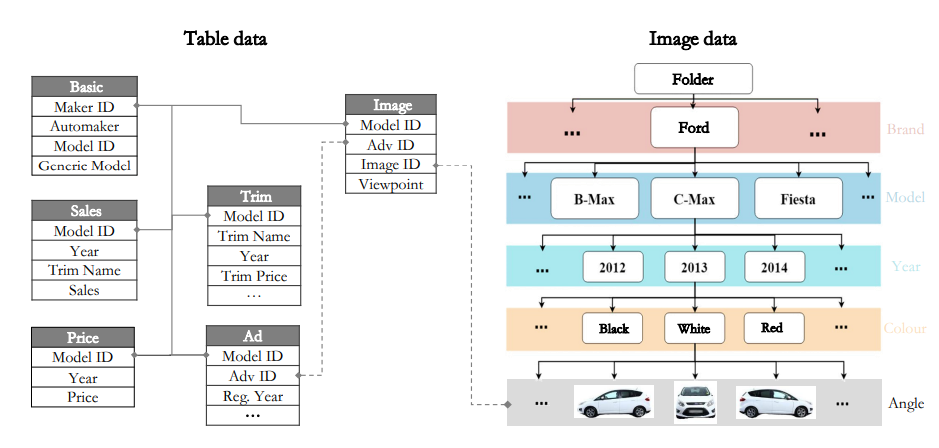
\includegraphics[width=1\linewidth]{general_data_tables.png}
        \end{figure}
    \end{frame}

    \begin{frame}{Data dictionary}
        \begin{figure}
         
        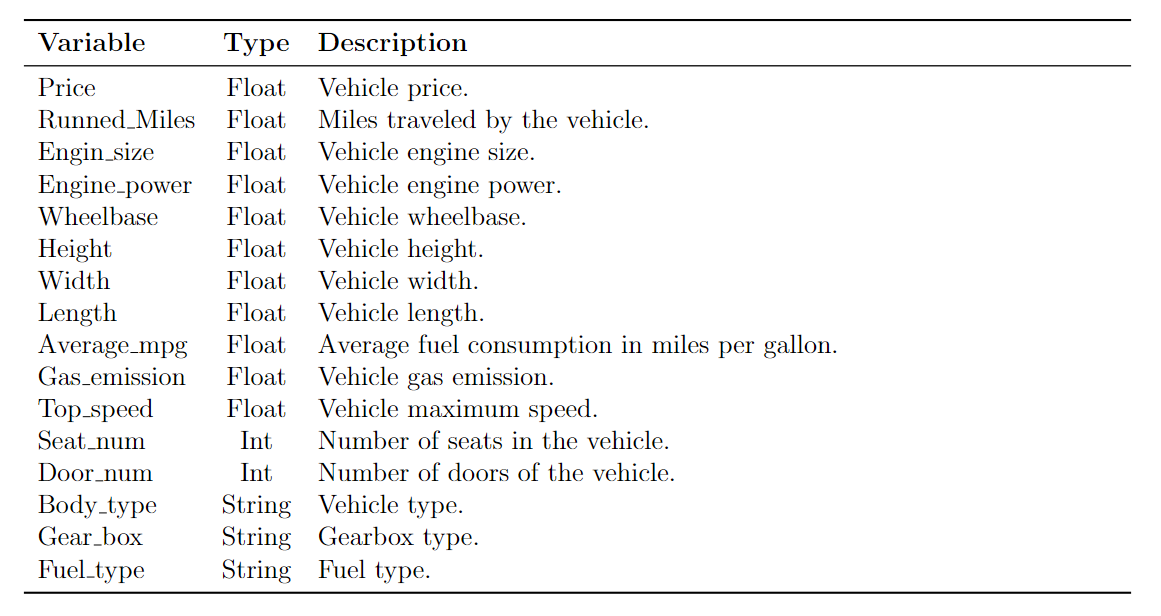
\includegraphics[width=0.9\linewidth]{data dictionary.png}
        \end{figure}
    \begin{itemize}
        \item Imputed missing values for \textit{Engine\_power}, \textit{Top\_speed}, \textit{Average\_mpg}, \textit{Engine\_size} \\[0.2 cm]    
    \end{itemize}
    \end{frame}

    \begin{frame}{Descriptive statistics} 
        \begin{itemize}
        \item 201K observations \\[0.2 cm]
        \item The variables \\[0.2 cm]
        \begin{itemize}
            \item The dependent variable : the price \\[0.1 cm]
            
            \item The independent variables : 33 categorical and numerical features \\[0.1 cm]
        \end{itemize}
        \begin{figure}
         
        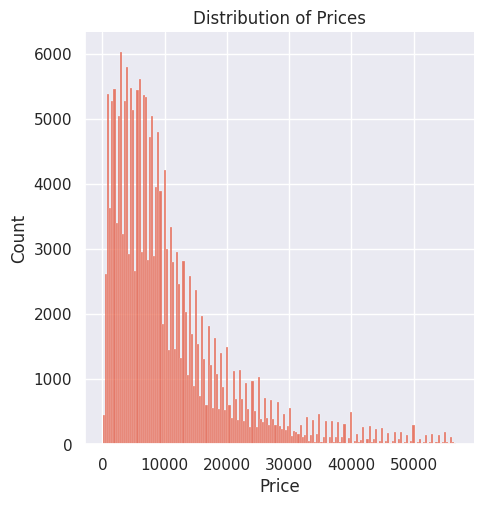
\includegraphics[width=0.4\linewidth]{distribution of prices.png}
        \caption{Distribution of prices}
        \end{figure}
    \end{itemize}
    \end{frame}

    

    \begin{frame}{Image Dataset} 
        
        \begin{figure}
        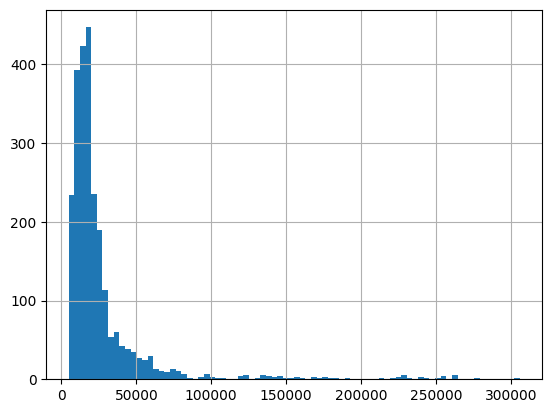
\includegraphics[width=0.35\linewidth]{price_image_distribution_1.png}
        \caption{Price image distribution with outliers}
        \end{figure}
        \begin{figure}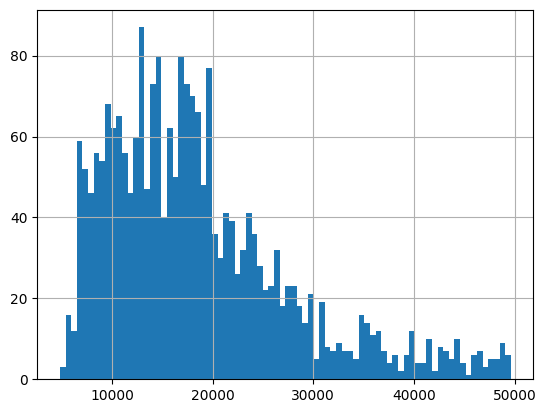
\includegraphics[width=0.35\linewidth]{price_image_distribution_2.png}
        \caption{Price image distribution without outliers}
        \end{figure}
    \end{frame}

\begin{frame}{Selected Machine Learning Models} 
    
    \begin{itemize}
        \item KNN \\[0.2 cm]
            \begin{itemize}
                \item Very simple benchmark model
                \item \cite{Samruddhi2020}: Promising results  for car price prediction
            \end{itemize}
            
            \item XGBoost \\[0.2 cm]
            \begin{itemize}
                \item Many hyperparameters allowing for refined tuning and regularization (less prone to overfitting)
                \item Powerful model often used as benchmark (\cite{flachaire2022}, \cite{Lolic2022})
                \item \cite{Gajera2021}: Promising results for car price prediction
            \end{itemize}
            
        \item MLP \\[0.2 cm]
        \begin{itemize}
                \item Design allows for complex input-output relationships
                \item \cite{Samruddhi2020}, \cite{Karakoç2020},\cite{Bilen2021}: ANN best model for car price prediction
            \end{itemize}
            
    \end{itemize}
    
\end{frame}

    \begin{frame}{Tuning KNN} 
    \begin{itemize}
        \item Finding the optimal k, that represents the number of neighbors \\[0.5 cm] 
        \begin{figure}[ht]
    \centering
    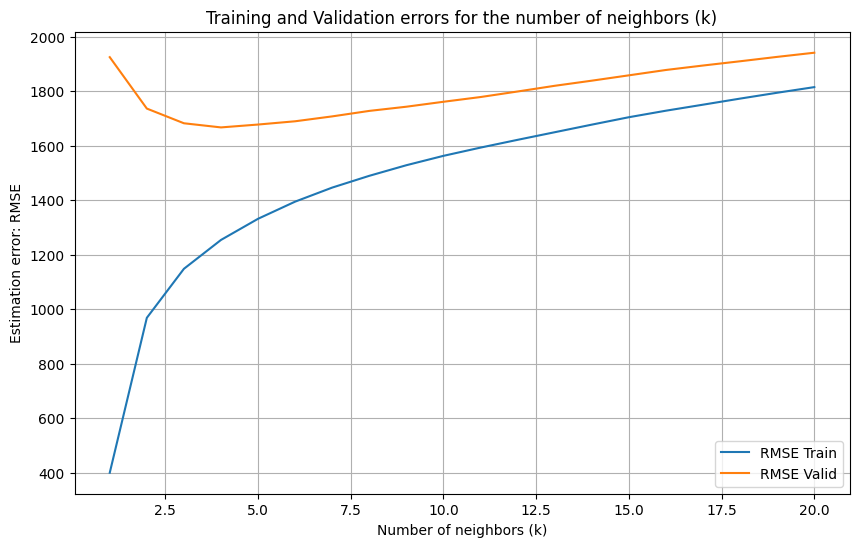
\includegraphics[width=0.45\textwidth]{Nb k.png}
    \caption{Training and Validation errors for the number of neighbors (k)}
    \label{Optimal k}
    \end{figure}
    \end{itemize}
    \end{frame}


    \begin{frame}{Tuning XGBoost: Tuning strategy} 

    \begin{itemize}
        \item Step-by-step tuning approach based on hyperparameter impact on model outcome:
            \begin{enumerate}
                \item Learning rate \& Number of Tree estimators
                \item Maximum tree depth \& minimum child weight
                \item Pruning parameter $\gamma$
                \item Regularization parameter $\lambda$
            \end{enumerate}
    \end{itemize}

    \begin{figure}[ht]
        \centering
        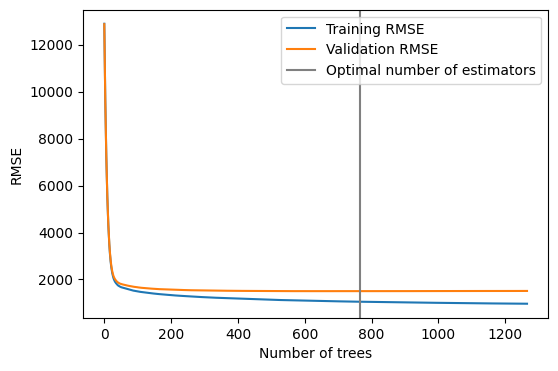
\includegraphics[width=0.4\textwidth]{xgb_num_estimators.png}
        \caption{Finding optimal number of estimators [$\eta = 0.1$]}
        \label{xgb_num_estimators}
    \end{figure}
\end{frame}


\begin{frame}{Tuning XGBoost: Model performance by tuning step}
\begin{figure}[ht]
    \centering
    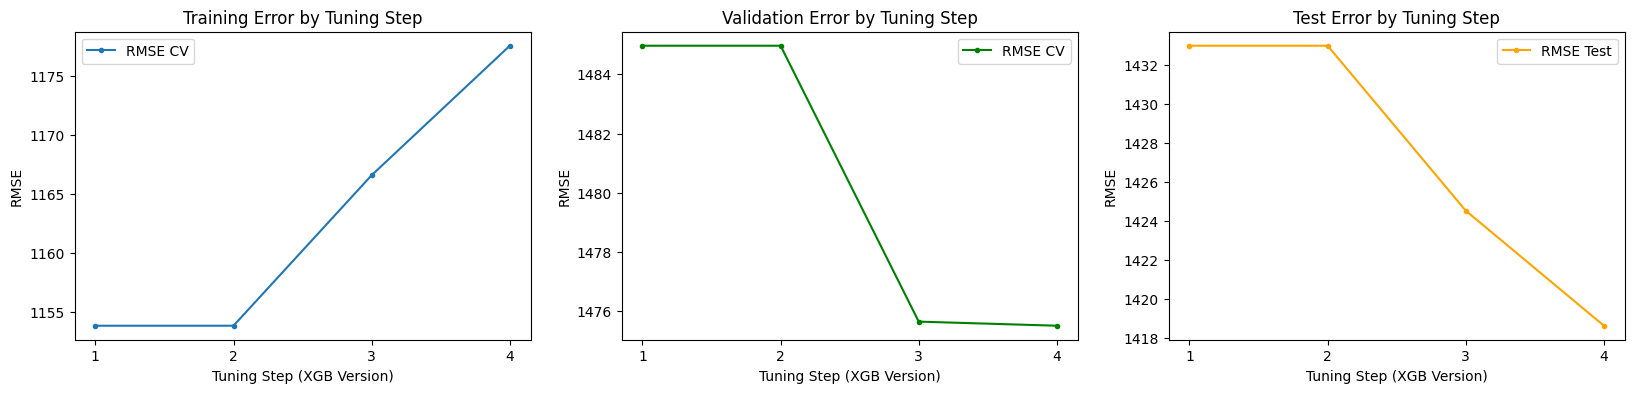
\includegraphics[width=0.9\textwidth]{rmse_evaluation.png}
    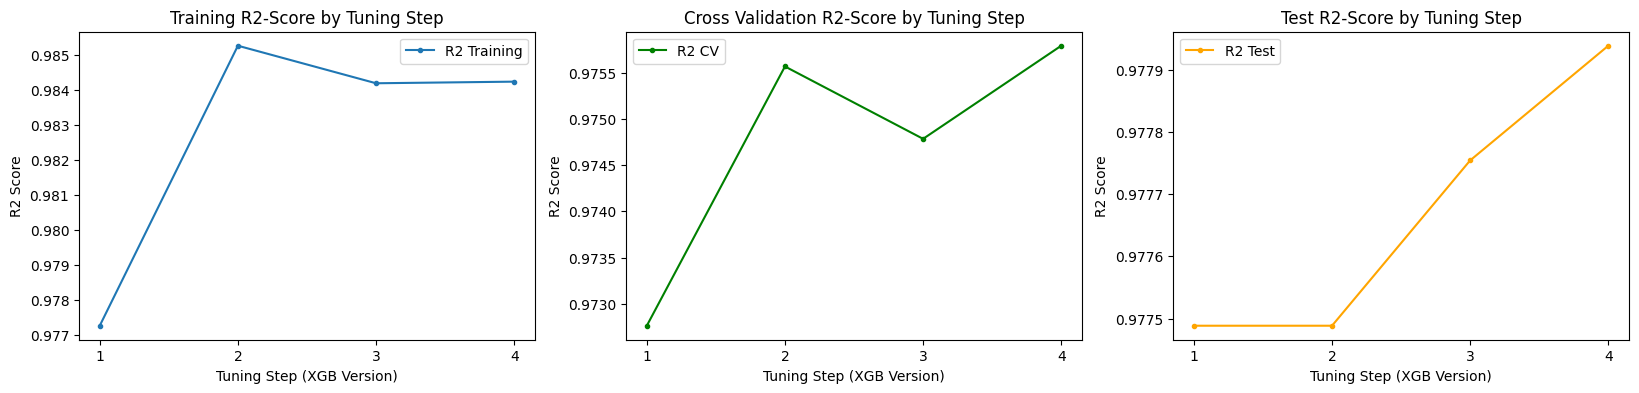
\includegraphics[width=0.9\textwidth]{r2_evaluation.png}
    \caption{Evaluation of RMSE and $R^2$ scores by tuning step}
    \label{performance_evaluation}
\end{figure}
\end{frame}


    \begin{frame}{Tuning XGBoost: Best estimator}
    \begin{table}[h]
        \centering
        \caption{Hyperparameters selected after 216 fits}
        \label{table:Parameters of the best MLP model}
    
        \begin{tabular}{lrrrrrrr}
        \toprule
        \textbf{Parameter} & \textbf{Value} \\
        \midrule
        Num. of tree estimators & 765\\
        Max. tree depth & 7\\
        Min. child weight & 1 \\
        Pruning param. $\gamma$ & 0 \\
        Regularization $\lambda$ & 1.5 \\
        \bottomrule
        \end{tabular}
    \end{table}
    \end{frame}






    \begin{frame}{Tuning MLP} 
        \vspace{0.5cm} % Adjust the amount of space as needed
        \begin{figure}[ht]
            \centering
            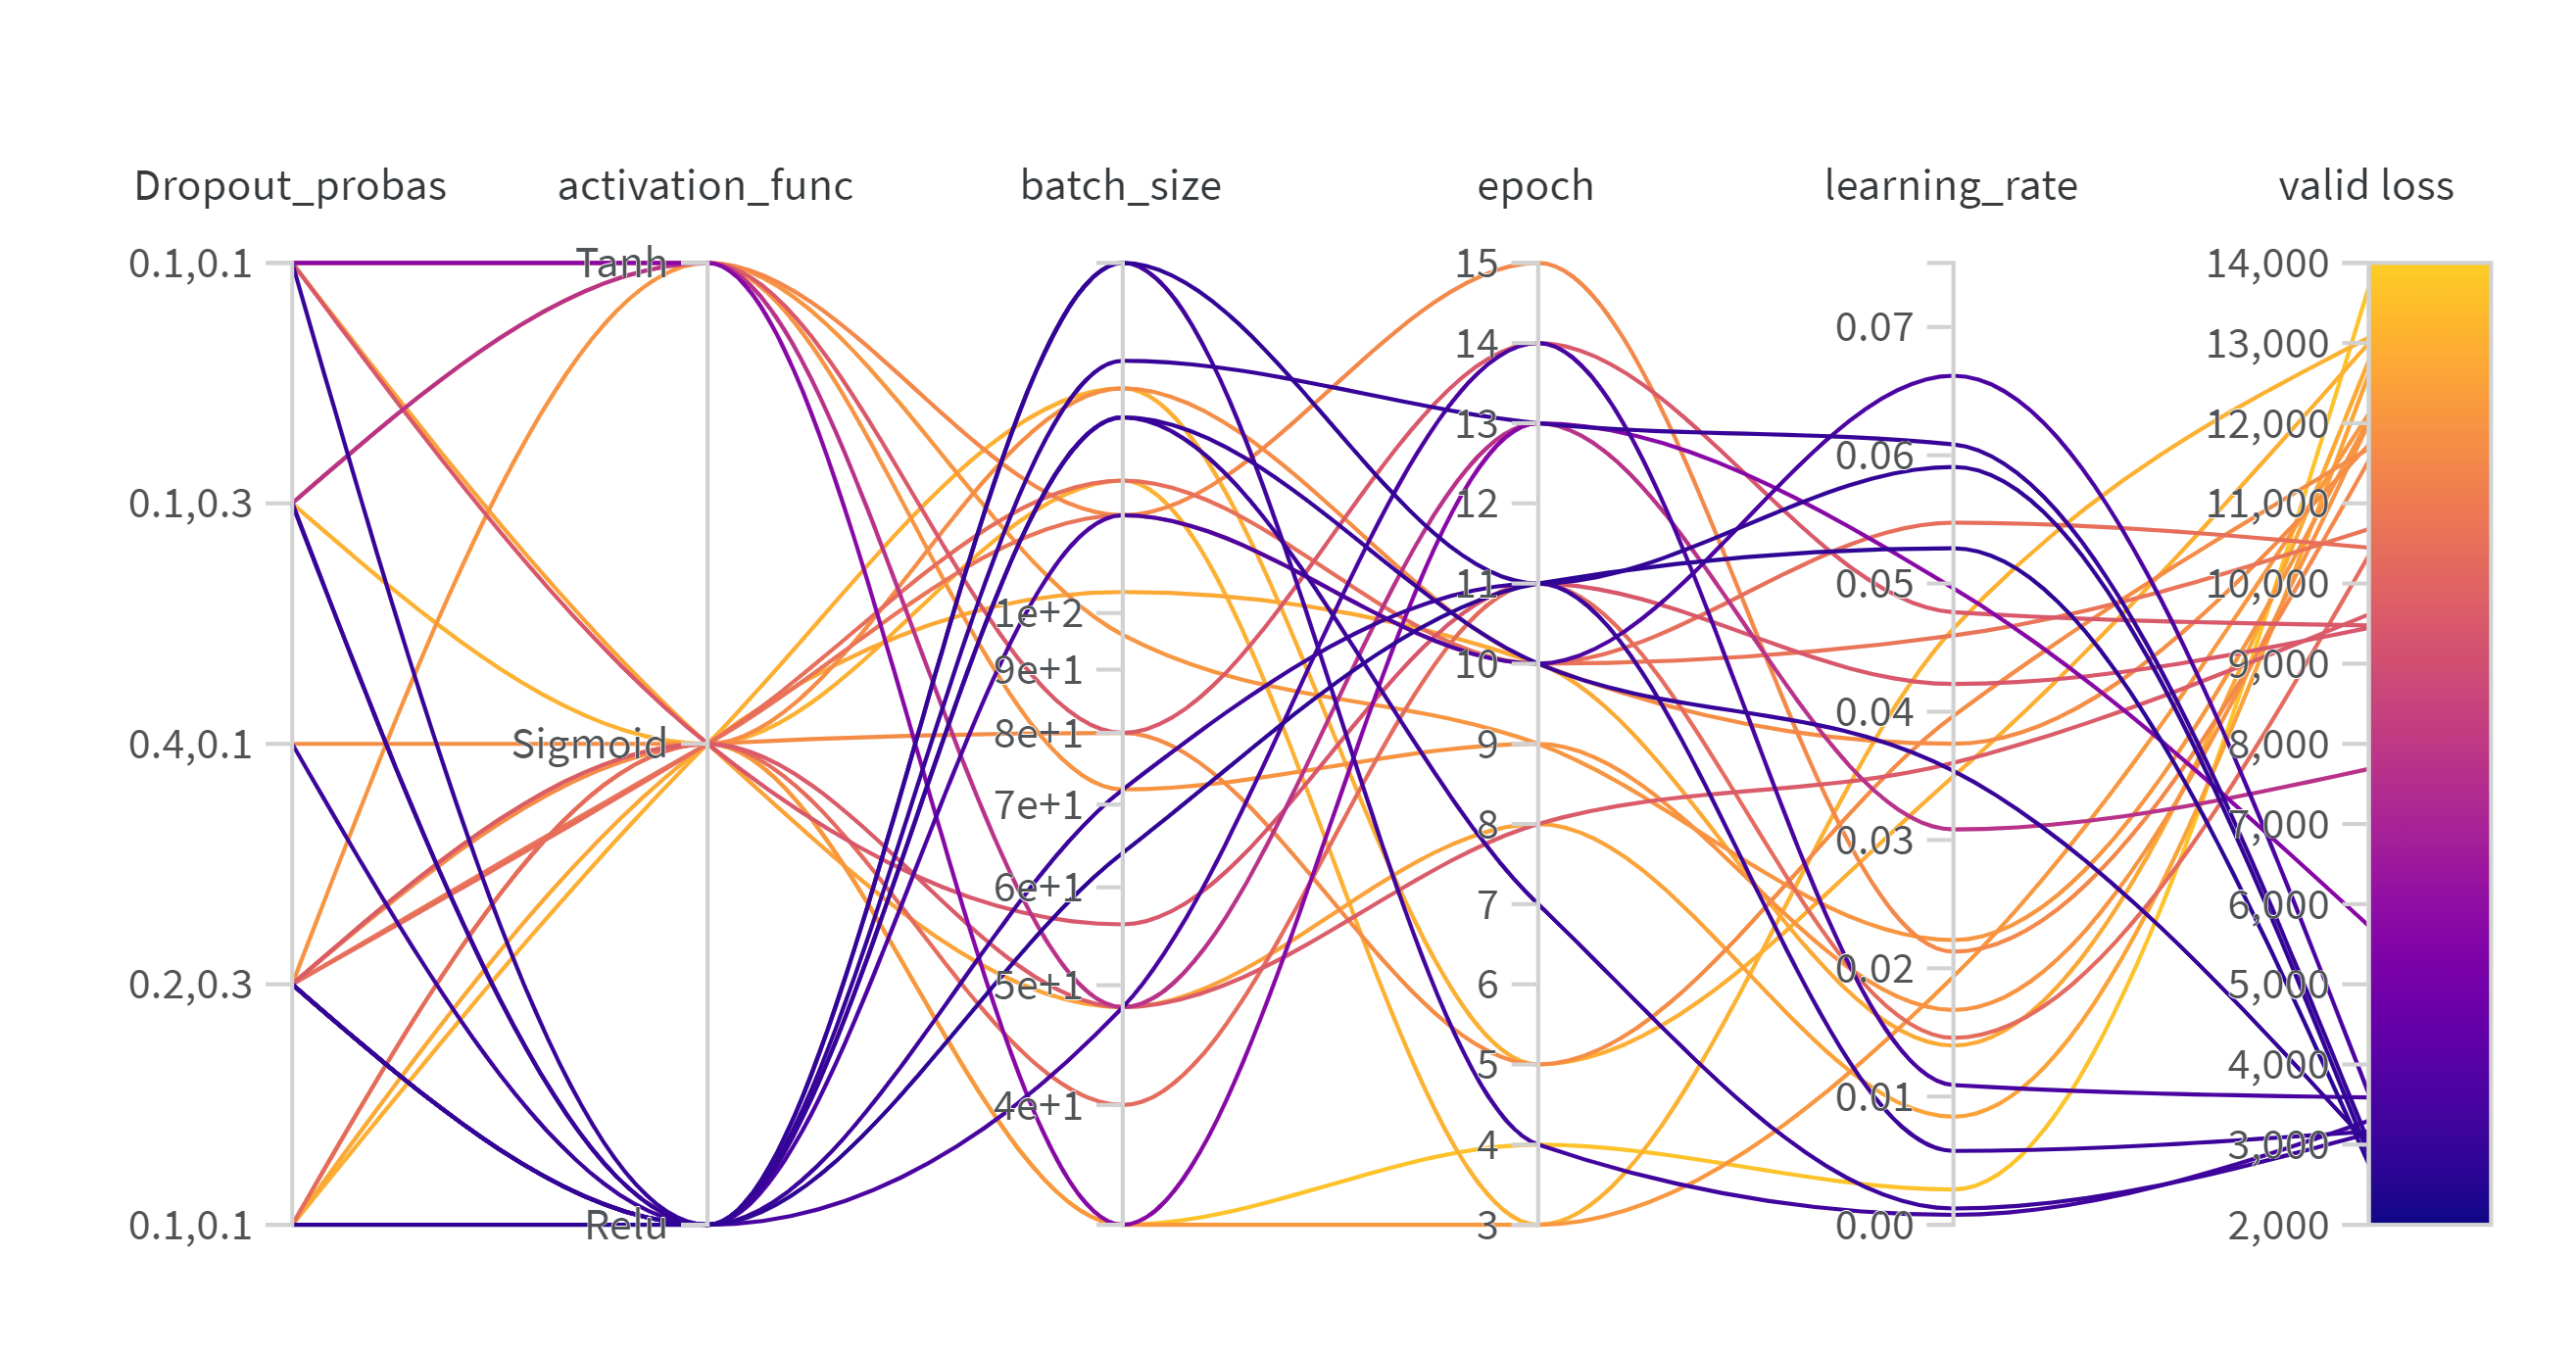
\includegraphics[width=1\textwidth]{wandbrun_1.png}
            \caption{Hyper parameters tuning results}
            \label{fig:HyperparametersTuningResults}
        \end{figure}
    \end{frame}

    \begin{frame}{Tuning MLP}
    \begin{table}[h]
        \centering
        \caption{Parameters selected after 30 runs}
        \label{table:Parameters of the best MLP model}
    
        \begin{tabular}{lrrrrrrr}
        \toprule
              \textbf{Parameter} & \textbf{Value} \\
        \midrule
        Batch Size & 64\\
        Learning Rate & 0.05274\\
        Activation Function & Relu \\
        Number of Input Features & 33 \\
        Total Number of Layers & 5 \\
        Sizes of Each Layer & 30, 25, 20, 10 \\
        Dropout probabilities & 0.1, 0.1, 0.1, 0.1 \\
        \bottomrule
        \end{tabular}
    \end{table}
    \end{frame}
    
    \begin{frame}{Tuning MLP}

    \begin{figure}[!h]
      \centering
      \begin{subfigure}{0.4\textwidth}
        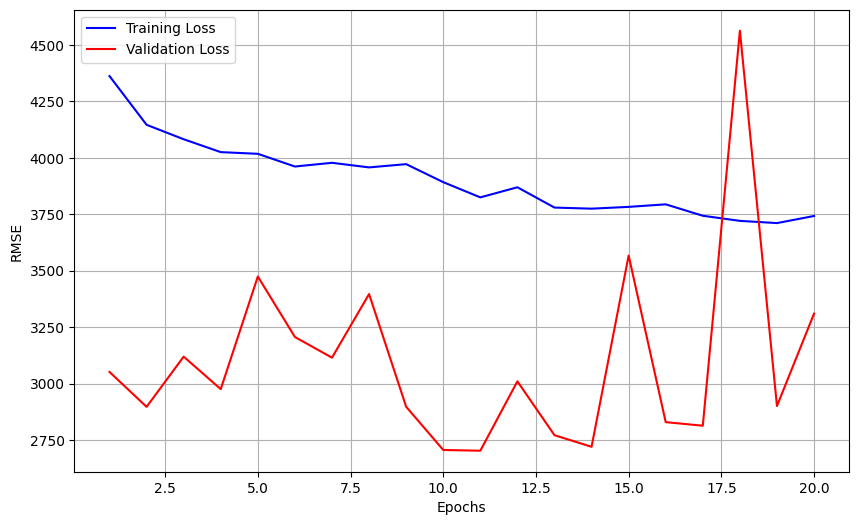
\includegraphics[width=\linewidth]{Training and Validation Loss with dropout probabilities.png}
        \caption{Training and Validation Loss with dropout probabilities}
        \label{Training and Validation Loss with dropout probabilities}
      \end{subfigure}
      \medskip
      \begin{subfigure}{0.4\textwidth}
        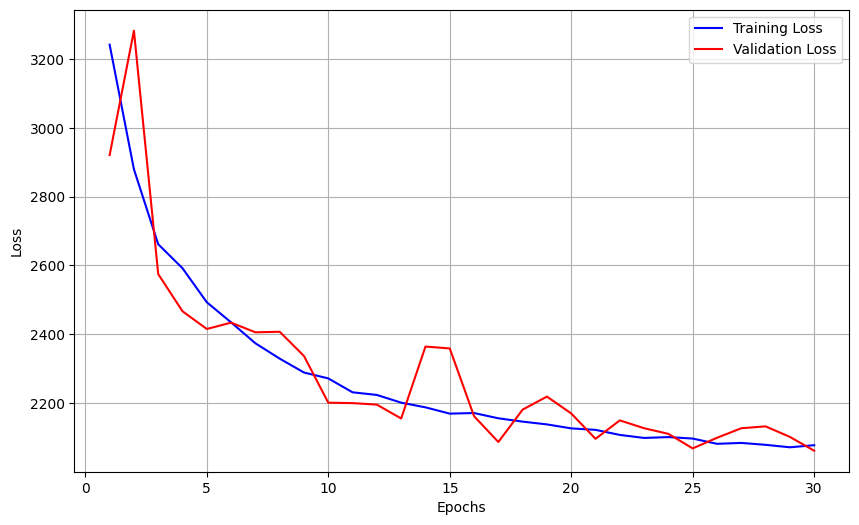
\includegraphics[width=\linewidth]{Training and Validation Loss without dropout probabilities.png}
        \caption{Training and Validation Loss without dropout probabilities}
        \label{Training and Validation Loss without dropout probabilities}
      \end{subfigure}
    \end{figure}
    
    \end{frame}

    \begin{frame}{Dimensionality reduction with Elastic Net} 
    \begin{itemize}
        \item Why elastic net?\footnote{Despite the advantages of the elastic net, applying it to the XGBoost will most certainly yield no better results due to the XGBoost design.}
            \begin{itemize}
                \item Facing high dimensional data (33 features) with strong collinearity among feature groups (e.g. car dimensions or engine specs)
                \item Feature selection independent from feature correlation   
            \end{itemize}
        \item Best estimator after 100 fits\footnote{based on four-fold cross validation}
            \begin{itemize}
                \item L1 regularization $\lambda_{1}= 0.9$
                \item L2 regularization $\lambda_{2}= 0.1$
            \end{itemize}
        \item Model performance
            \begin{itemize}
                \item $RMSE = 4497.61$
                \item $R^{2} = 0.7782$
            \end{itemize}
    \end{itemize}
    
       
    \end{frame}

    \begin{frame}{Dimensionality reduction with PCA} 
        
    \begin{itemize}
        \item Why PCA ?
    \begin{figure}[ht]
        \centering
        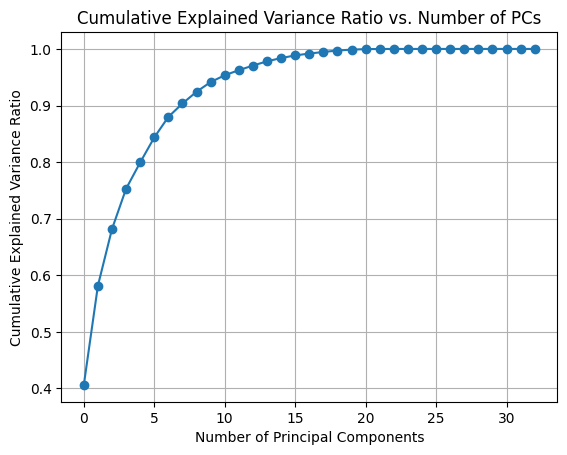
\includegraphics[width=0.45\textwidth]{PCA.png}
        \caption{Number of Components}
        \label{PCA}
    \end{figure}
    \item We selected 11 Components, that captures 95\% of the variance
    \end{itemize}
    \end{frame}

    \begin{frame}{Comparison results} 

    \begin{table}[h]
    \centering
    \caption{Model comparison}

    \begin{tabular}{lccc}
        \toprule
        \textbf{Model} & \multicolumn{2}{c}{\textbf{RMSE}} \\
         & \textbf{Training} & \textbf{Test} \\
        \midrule
        \textbf{KNN} & 1254.05 & 1719.35 \\
        \textbf{KNN + PCA} & 1272.46 & 1735.86 \\
        \textbf{XGBOOST} & \textbf{1178.93} & \textbf{1418.60} \\
        \textbf{XGBOOST + Elastic Net} & 1185.53 & 1443.99 \\
        \textbf{MLP} & 2077.84 & 2057.50 \\
        \textbf{MLP + PCA} & 2983.15 & 3056.08 \\
        \bottomrule
    \end{tabular}
    \label{Model_comparison}
    \end{table}
      
    \end{frame}


    
    \begin{frame}{Model-Agnostic methods: SHAP}
    \begin{figure}[ht]
        \centering
        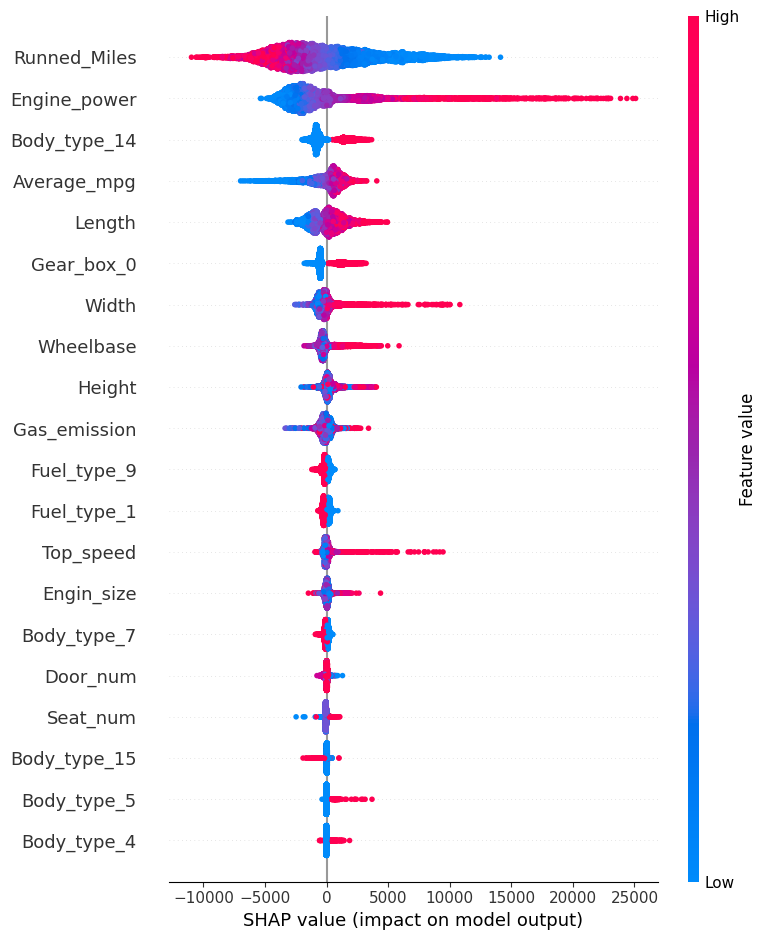
\includegraphics[width=0.5\textwidth]{xgboostshapely.png}
        \caption{Beeswarm shapley graph of XGBoost predictions}
        \label{xgboostshapley}
    \end{figure}
    \end{frame}

\begin{frame}{Model-Agnostic methods: PDP \& ICE plots}
  \begin{figure}[h]
    \centering
    \begin{subfigure}{0.38\textwidth}
      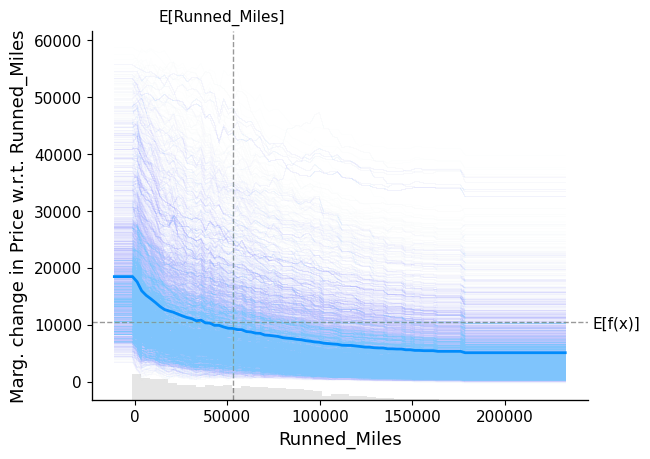
\includegraphics[width=\linewidth]{ice_runnedmiles.png}
      \caption{ICE Plots for Mileage}
      \label{ice_runnedmiles}
    \end{subfigure}
    \hfill
    \begin{subfigure}{0.38\textwidth}
      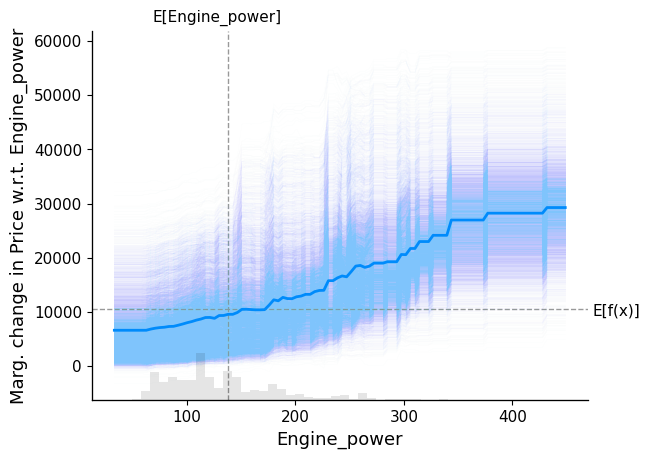
\includegraphics[width=\linewidth]{ice_enginepower.png}
      \caption{ICE Plots for Engine Power}
      \label{ice_enginepower}
    \end{subfigure}

    \medskip

    \begin{subfigure}{0.38\textwidth}
      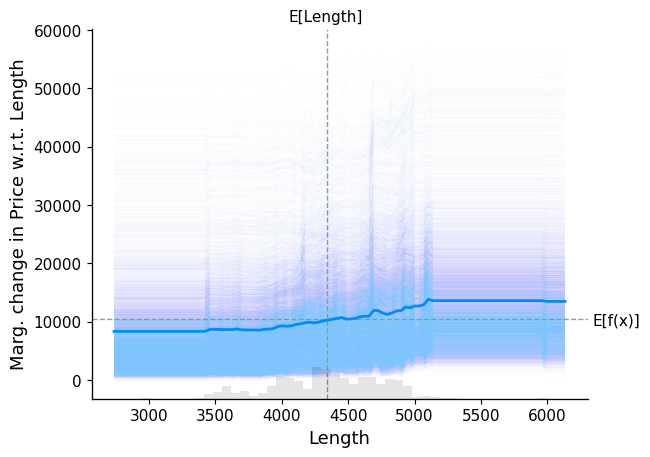
\includegraphics[width=\linewidth]{ice_length.png}
      \caption{ICE Plots for Length}
      \label{ice_length}
    \end{subfigure}
    \hfill
    \begin{subfigure}{0.38\textwidth}
      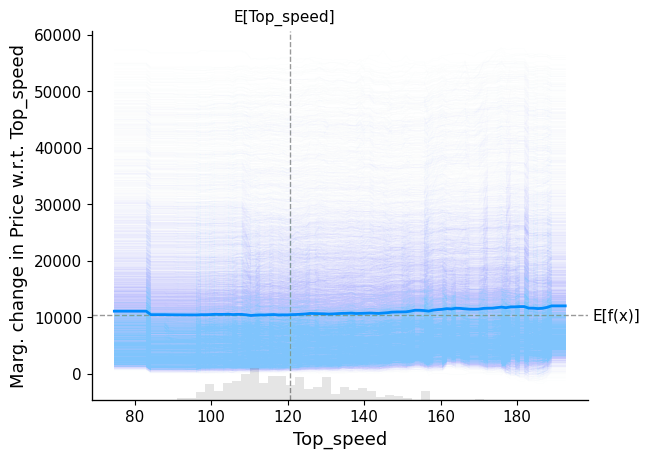
\includegraphics[width=\linewidth]{ice_topspeed.png}
      \caption{ICE Plots for Top Speed}
      \label{ice_topspeed}
    \end{subfigure}
    
    \caption{Independent Conditional Expectation Plots}
    \label{ice_plots}
  \end{figure}
\end{frame}




    \begin{frame}{CNN} 
    
    \begin{figure}[ht]
        \centering
        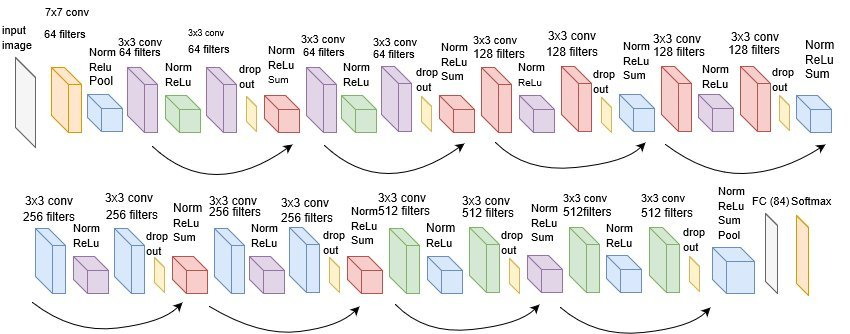
\includegraphics[width=0.85\textwidth]{resnet18.jpeg}
        \caption{Resnet-18 architecture}
        \label{Resnet18}
    \end{figure}

    \end{frame}

    \begin{frame}{Data normalization and data augmentation} 
        

    \centering

    \begin{figure}[ht]
    \centering
    \label{table:images without transformations}
    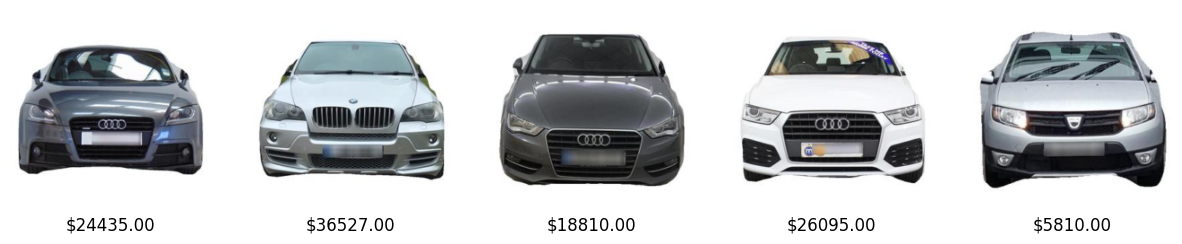
\includegraphics[width=0.6\textwidth]{images without transformations.png}
    \caption{Original images}
    \end{figure}

    \begin{figure}[ht]
    \centering
    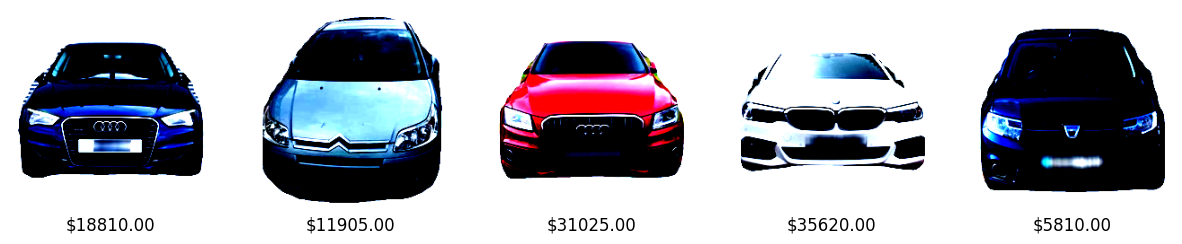
\includegraphics[width=0.6\textwidth]{testing images.png}
    \caption{Normalized images}
    \label{Normalized images}
    \end{figure}

    \begin{figure}[ht]
    \centering
    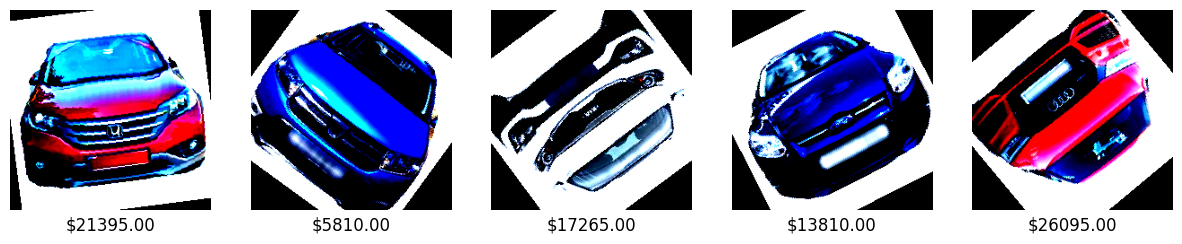
\includegraphics[width=0.6\textwidth]{training images.png}
    \caption{Rotated images}
    \label{training images}
    \end{figure}
    
    \end{frame}
    \begin{frame}{CNN} 

    \begin{figure}[ht]
        \centering
        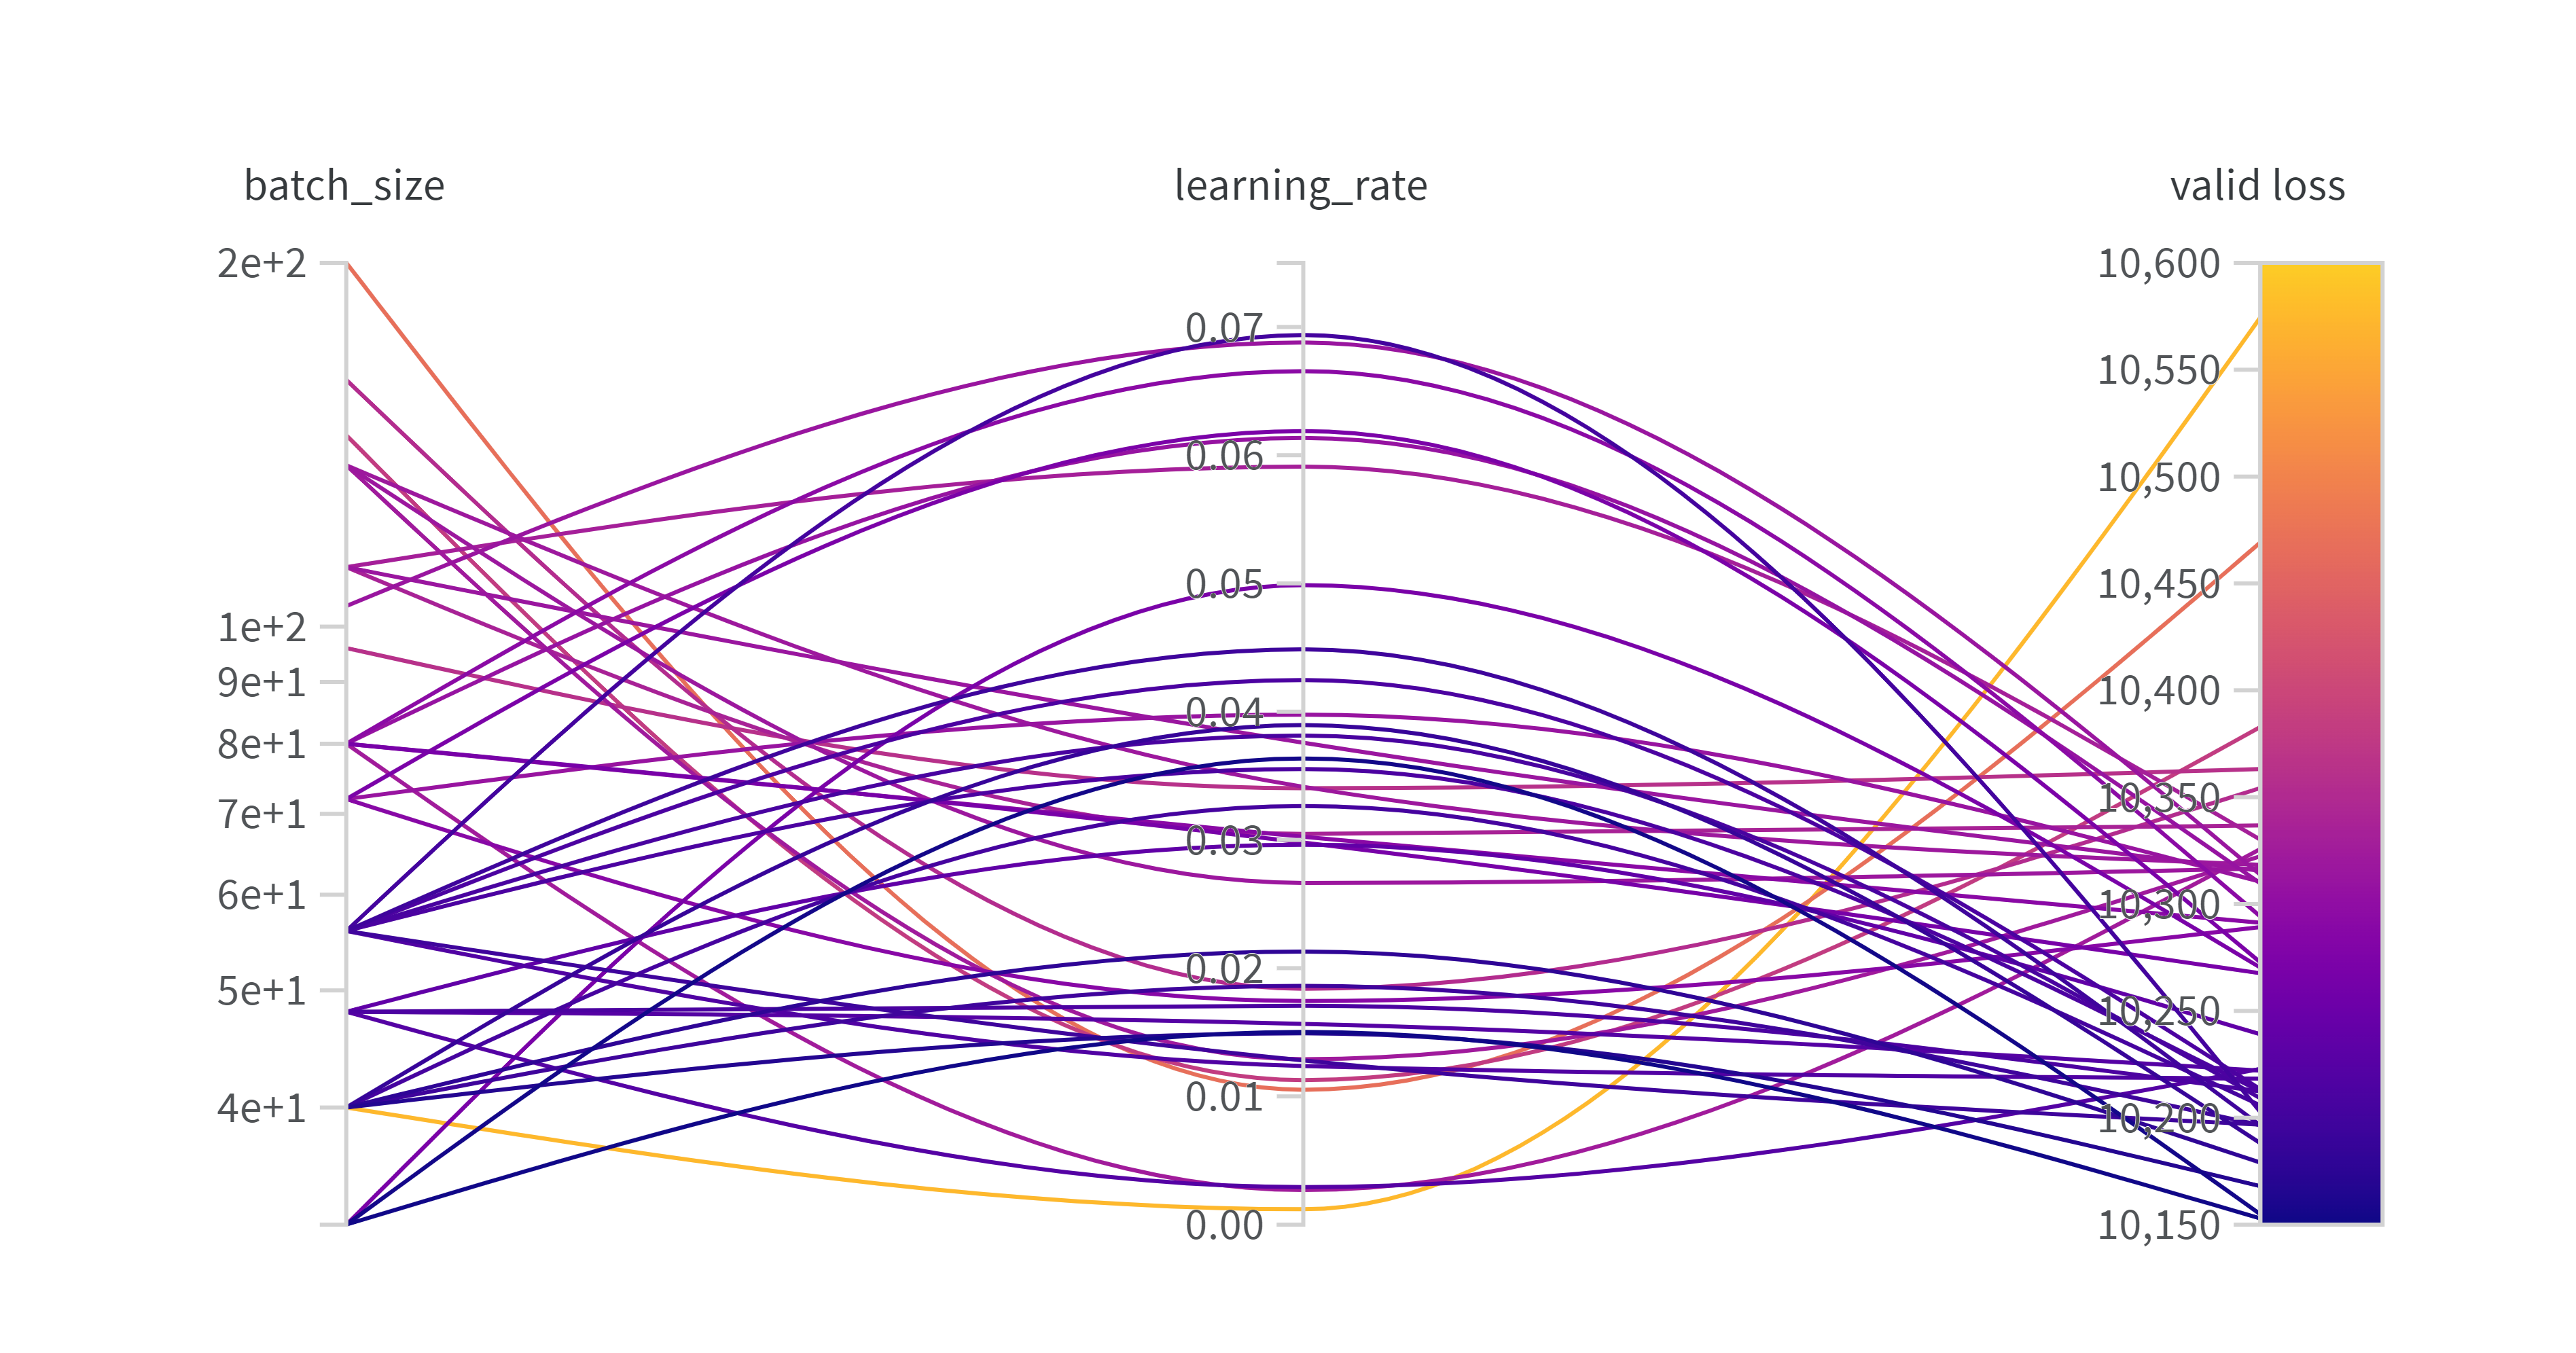
\includegraphics[width=0.9\textwidth]{cnn_wandb.png}
        \caption{Hyper parameters tuning results for the Resnet18}
        \label{Tuning CNN}
    \end{figure}
    \end{frame}
    
    \begin{frame}{CNN results}
    \begin{table}[h]
    \centering
    \caption{Results of the Resnet18 model}
    \label{Results CNN}
    \begin{tabular}{lrrrrrrr}
    \toprule
           & RMSE \\
    \midrule
    Train & 15945.92\\
    Validation & 10176.11\\
    Test & 10746.46\\
    \bottomrule
    \end{tabular}
    \end{table}
        
    \end{frame}



    \begin{frame}{Conclusion} 

    \begin{itemize}
        \item Results:
            \begin{itemize}
                \item XGBoost best model for car price prediction\footnote{These findings are in line with \cite{Pudaruth2014}, \cite{Gajera2021}}
                \item Most important features: Mileage, engine power, body type 14, average mpg and length
                \item Poor predicition based on image data
            \end{itemize}
        \item Limitations:
            \begin{itemize}
                \item Models limited to cars worth less than \$50,000
                \item Mispricing around \$1418.60 not acceptable for merchants and buyers
            \end{itemize}
        \item Further research suggestions:
            \begin{itemize}
                \item Development of specific models for certain price categories
                \item Apply deeper CNNs (Resnet50, Resnet101)
                \item Perform model concatenation
            \end{itemize}
    \end{itemize}
\end{frame}




\begin{frame}
  \begin{center}
    \Huge \textit{Thank you for your attention!}
  \end{center}
\end{frame}

\begin{frame}{References}
  \begin{center}
    \printbibliography
  \end{center}
\end{frame}



    \begin{frame}{Q\&A} 
        
        \begin{figure}
         
        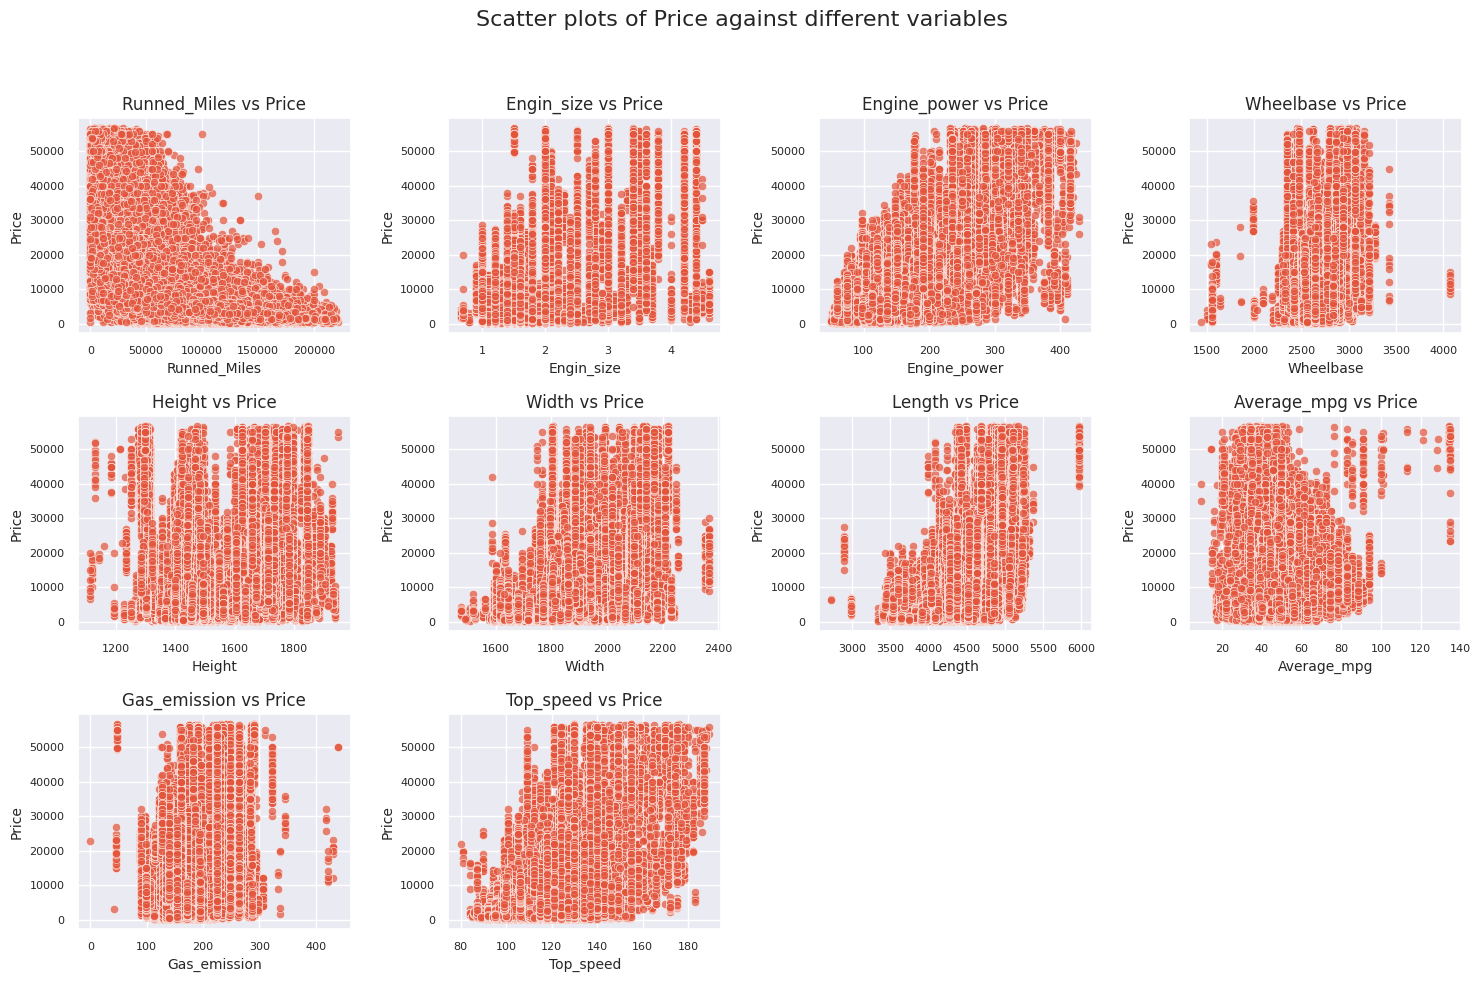
\includegraphics[width=0.8\linewidth]{numerique variables.png}
        \caption{Relationship between numerical variables and the price}
        \end{figure}
    \end{frame}

\begin{frame}{Q\&A}
\begin{figure}[ht]
    \centering
    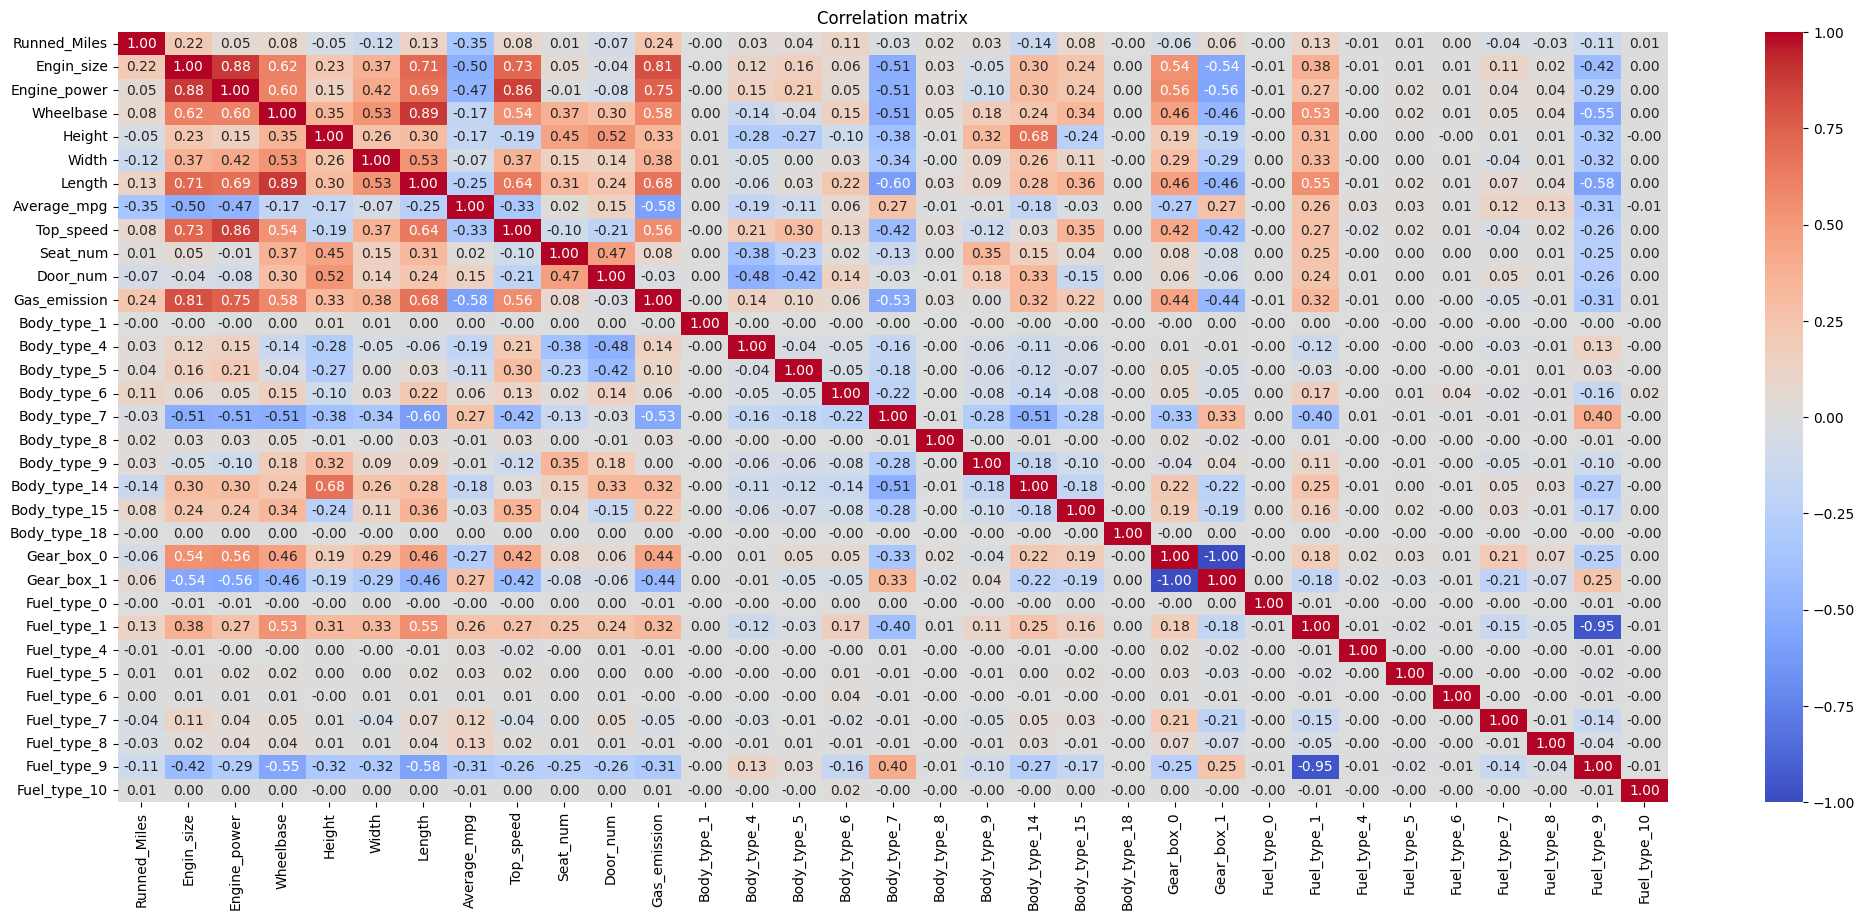
\includegraphics[width=0.90\textwidth]{Correlation matrix.png}
    \caption{Correlation matrix}
    \label{Correlation matrix}
\end{figure}
\end{frame}




\begin{frame}{Q\&A}
    \begin{figure}[ht]
        \centering
        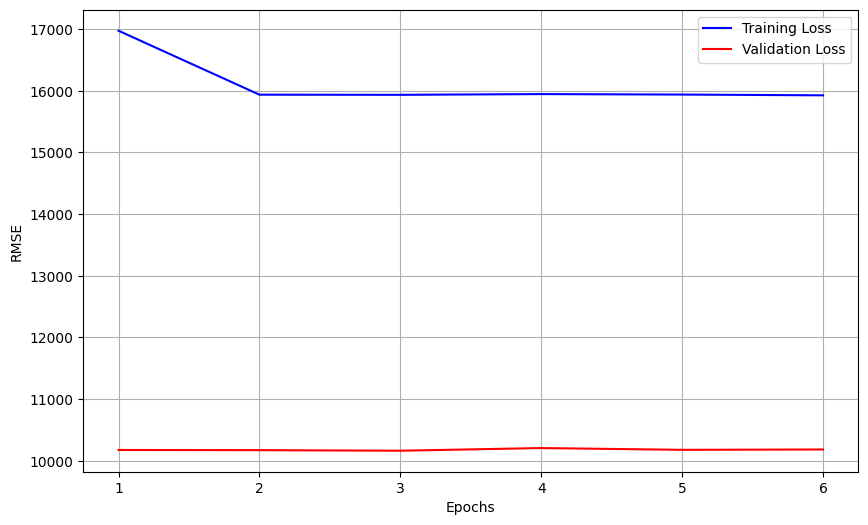
\includegraphics[width=0.5\textwidth]{training CNN.png}
        \caption{training CNN}
        \label{Training CNN}
    \end{figure}

    \end{frame}


    \begin{frame}{Q\&A}
    \begin{figure}[ht]
        \centering
        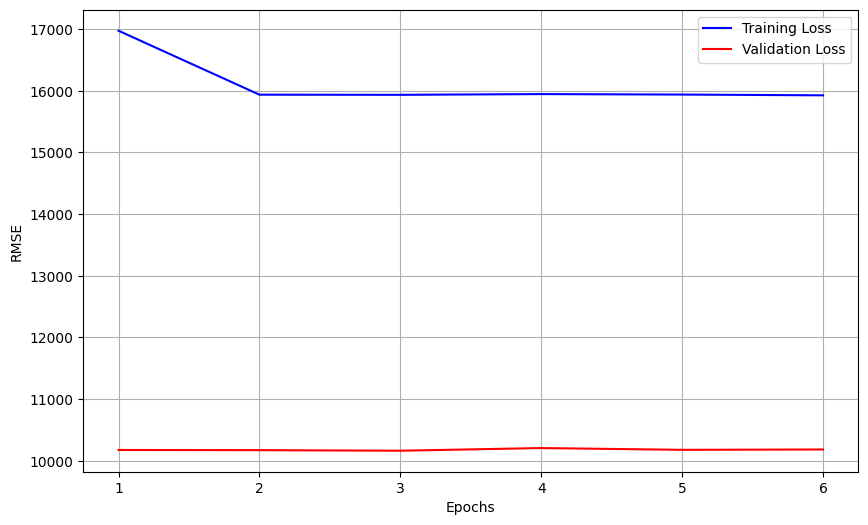
\includegraphics[width=0.5\textwidth]{training CNN.png}
        \caption{training CNN}
        \label{Training CNN}
    \end{figure}

    \end{frame}
    
    \begin{frame}{Q\&A}

    \begin{figure}[ht]
        \centering
        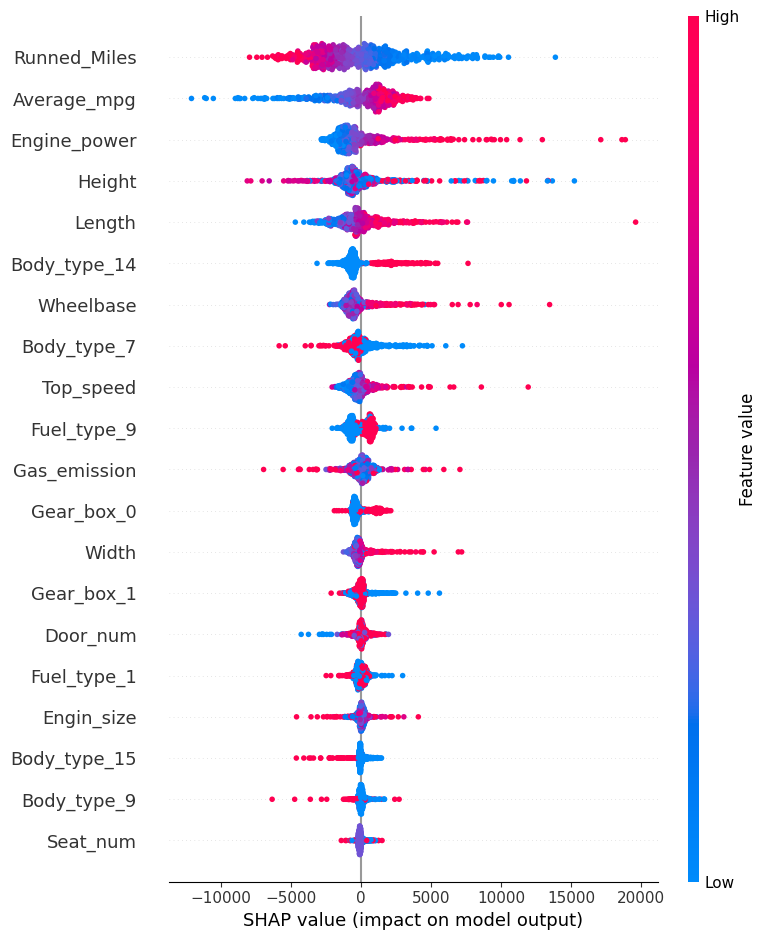
\includegraphics[width=0.5\textwidth]{shap MLP.png}
        \caption{Shapley values graph of MLP predictions}
        \label{shap MLP}
    \end{figure}
    \end{frame}

    \begin{frame}{Q\&A}
    \begin{table}[h]
        \centering
        \caption{Parameters swapped through a distribution function}
        \label{table:Parameters swapped through a distribution function}
        \begin{tabular}{lrrrrrrr}
        \toprule
               & Minimum & Maximum & Distribution \\
        \midrule
         Learning rate & 0.0005 & 0.07 & Uniform  \\
         Batch size & 30 & 200 & Q\_log\_Uniform  \\
         Epoch & 3 & 15 & Q\_log\_Uniform  \\
        \bottomrule
        \end{tabular}
    \end{table}
    \end{frame}

    
    \begin{frame}{Q\&A}
    \begin{table}[h]
        \centering
        \caption{Parameters swapped with limited sets}
        \label{table:Parameters swapped with limited sets}
    
        \begin{tabular}{lrrrrrrr}
        \toprule
               & \textbf{Set of possible values} \\
        \midrule
         \textbf{Activation function} & \begin{tabular}[c]{@{}l@{}}Tanh\\ Sigmoid\\ Relu\end{tabular} \\
         \textbf{Dropout probabilities} & \begin{tabular}[c]{@{}l@{}}0.1, 0.1, 0.1, 0.1\\
                                     0.3, 0.2, 0.1, 0.1\\
                                     0.1, 0.1, 0.2, 0.3\\
                                     0.1, 0.4, 0.4, 0.1\\
                                     0.3, 0.1, 0.1, 0.3\end{tabular} \\
        \bottomrule
        \end{tabular}
    \end{table}
    \end{frame}


\end{document}

